\documentclass{article}

\usepackage{graphicx} % Required for inserting images
\usepackage{verbatim}
\usepackage[utf8]{inputenc}
\usepackage{graphicx}
\usepackage{float}
\usepackage{fancyvrb}
\usepackage{varwidth}
\usepackage{amsmath}
\usepackage{siunitx}
\usepackage{caption}
\usepackage{subcaption}


\title{Speech Processing\\EE679}
\author{Mohit\\20D070052 }
\date{September 2023}

\begin{document}

\maketitle
\begin{figure}[H]
\begin{center}

\includegraphics[scale = 0.2]{LOGO.jpeg}
\end{center}
\end{figure}
\section{Student Details}
\begin{tabular}{ l l  }
 Name: & Mohit \\ 
 Roll No: & 20D070052  \\  
\end{tabular}

\newpage

\section{Question}

Use your previous synthesized vowel /u/ at two distinct pitches (F0 = 120 Hz, F0 = 220 Hz). Keep the bandwidths constant at 100 Hz for all formants. \\
Vowel F1, F2, F3 \\
/u/ 300, 870, 2240\\
We would like to use the DFT computed with various window lengths and shapes to estimate the vowel’s F0 and formant frequencies and study the obtained accuracies with reference to our ‘ground truth’ values. For the analysis, use a single waveform segment near the centre of your synthesized vowel. Plot the magnitude (dB) spectrum with rectangular and Hamming windows of lengths: 5 ms, 10 ms, 20 ms, 40 ms, each with a large zero-padded DFT. (i) Comment on the similarities and differences between the different computed spectra. (ii) Estimate the signal parameters from each of the magnitude spectra and report the error with respect to the ground-truth.

\subsection{Solution}
Building upon the code of the Question 4 of Assignment 1A, we will modify the code to include the Hamming and Rectangular Window Responses to Compare with the Ground Truth Values. Here we will show the plots obtained using different window lengths.

\subsection{Code}
The code files are included in the .ipynb file included in the submission.

\subsection{Plots}

\begin{figure}[H]
\centering
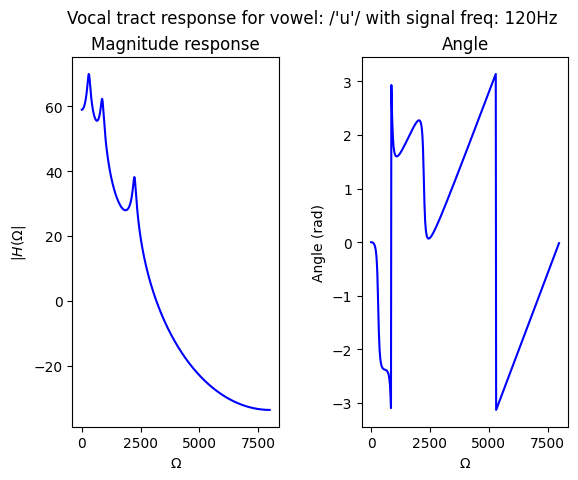
\includegraphics[scale = 0.5]{Q4_C1.png}
\caption{Original Magnitude Response and Phase Response}
\end{figure}
\newpage

\begin{figure}[H]
\centering
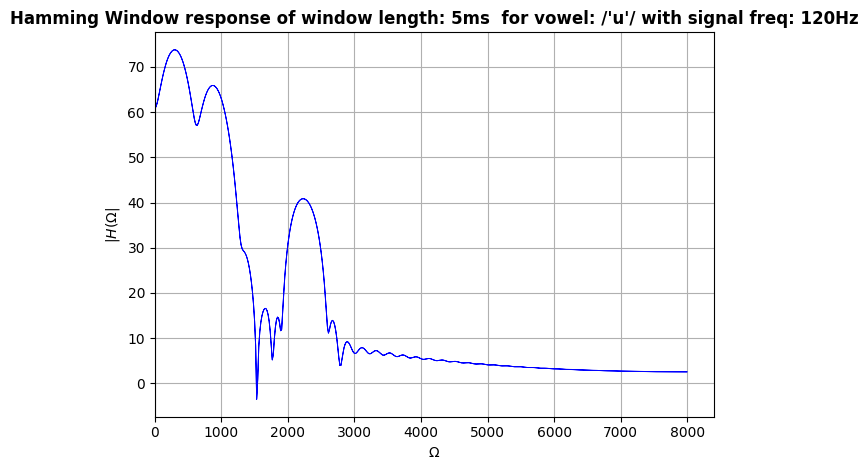
\includegraphics[scale = 0.5]{ham_5_120.png}\hfill
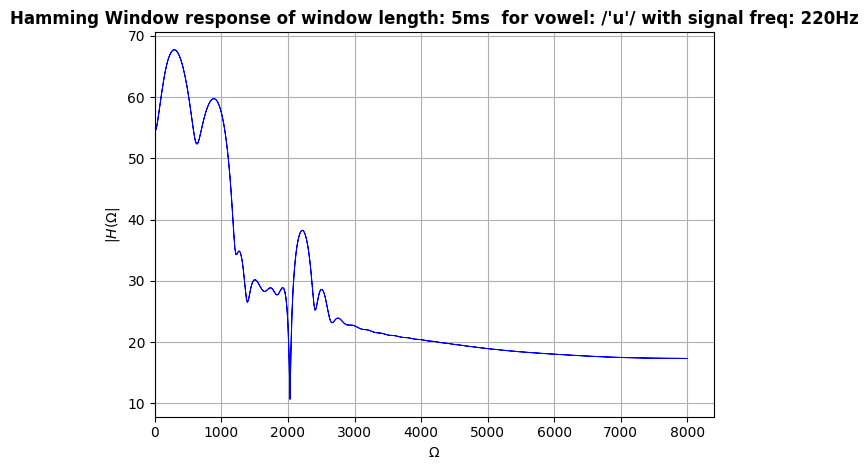
\includegraphics[scale = 0.5]{ham_5_220.png}
\caption{Hamming Window of 5ms at Different F0}
\end{figure}

\begin{figure}[H]
\centering
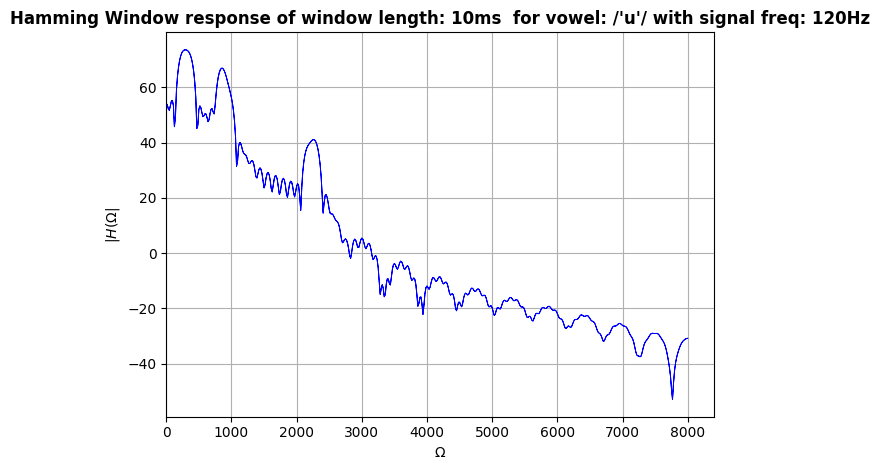
\includegraphics[scale = 0.5]{ham_10_120.png}\hfill
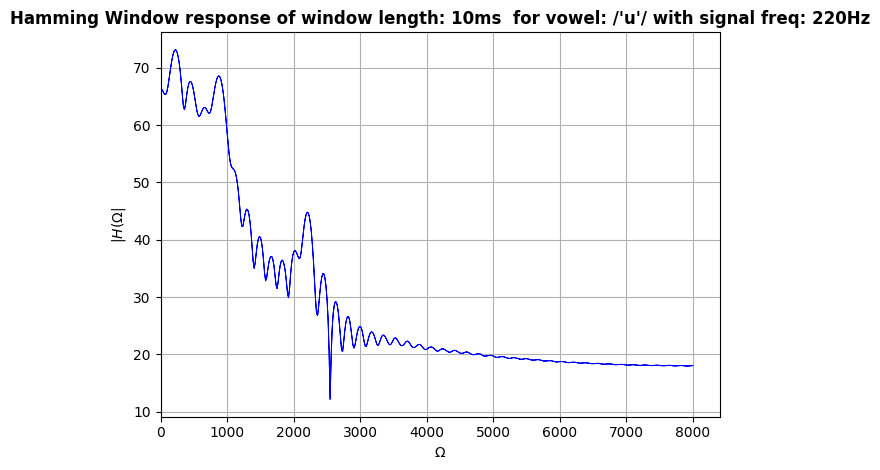
\includegraphics[scale = 0.5]{ham_10_220.png}
\caption{Hamming Window of 10ms at Different F0}
\end{figure}
\newpage

\begin{figure}[H]
\centering
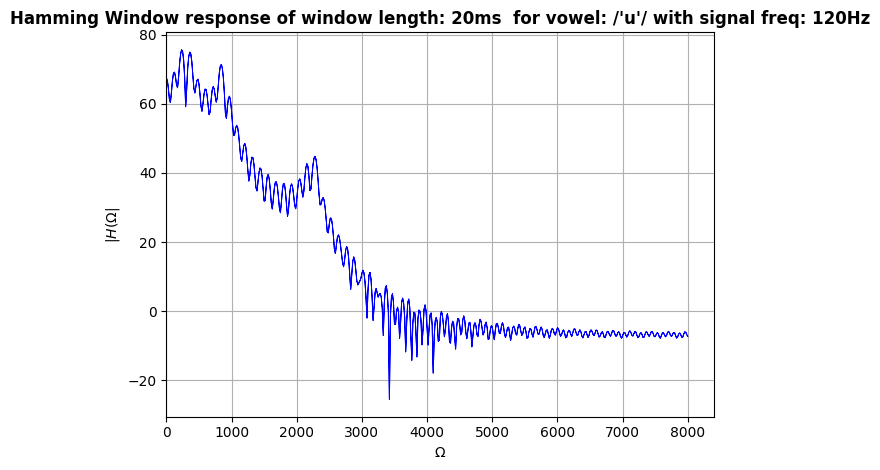
\includegraphics[scale = 0.5]{ham_20_120.png}\hfill
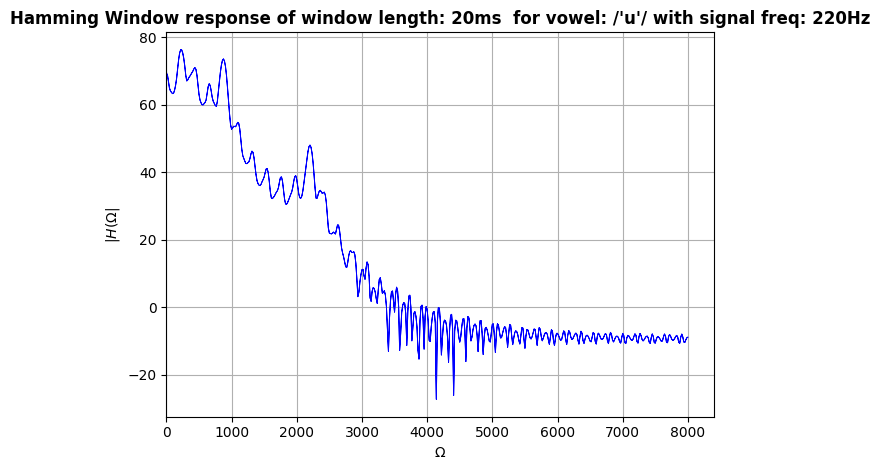
\includegraphics[scale = 0.5]{ham_20_220.png}
\caption{Hamming Window of 20ms at Different F0}
\end{figure}

\begin{figure}[H]
\centering
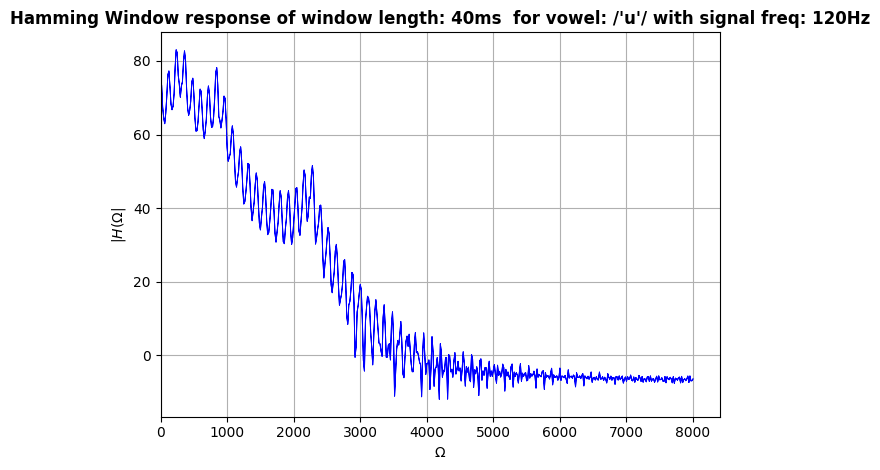
\includegraphics[scale = 0.5]{ham_40_120.png}\hfill
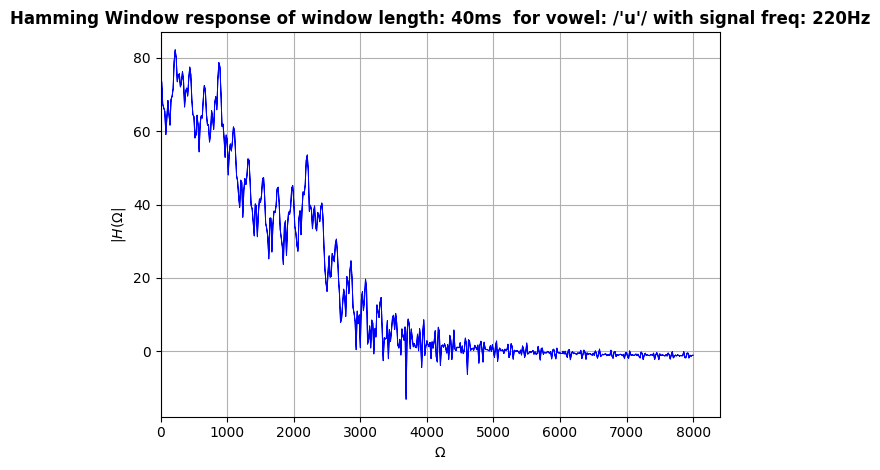
\includegraphics[scale = 0.5]{ham_40_220.png}
\caption{Hamming Window of 40ms at Different F0}
\end{figure}
\newpage

\begin{figure}[H]
\centering
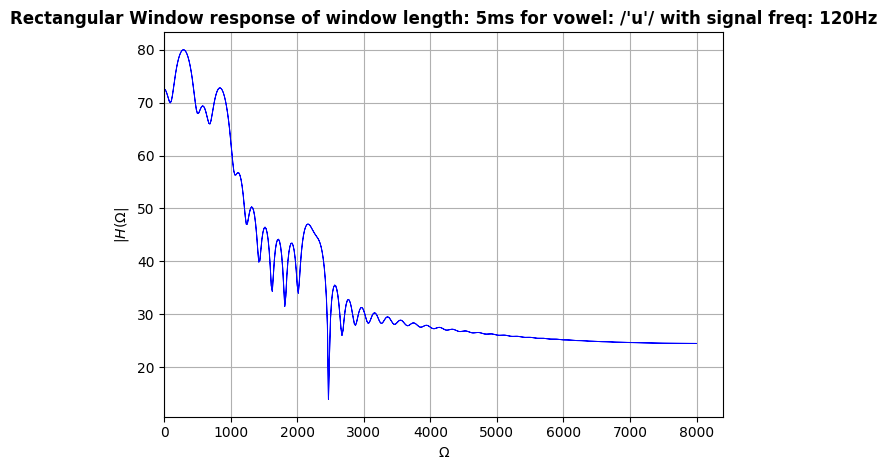
\includegraphics[scale = 0.5]{rect_5_120.png}\hfill
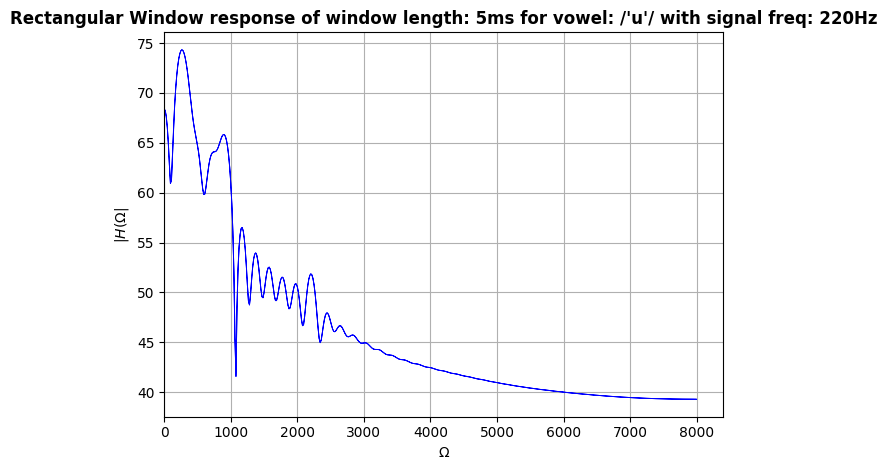
\includegraphics[scale = 0.5]{rect_5_220.png}
\caption{Rectangular Window of 5ms at Different F0}
\end{figure}

\begin{figure}[H]
\centering
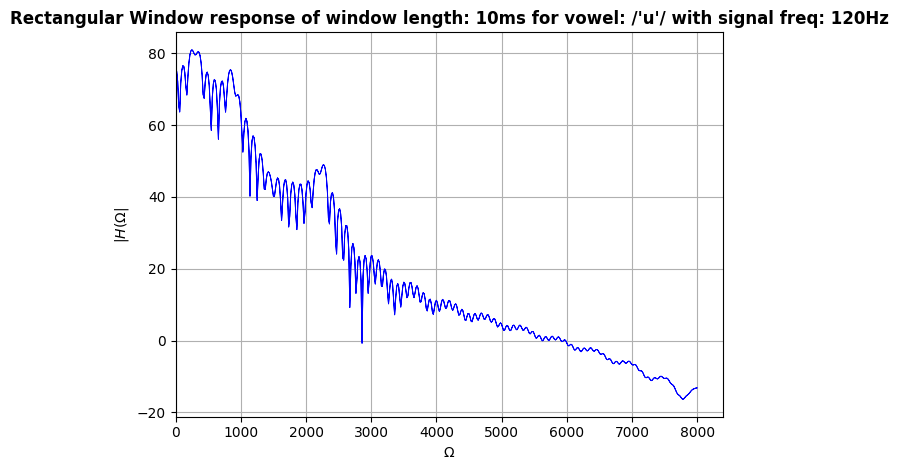
\includegraphics[scale = 0.5]{rect_10_120.png}\hfill
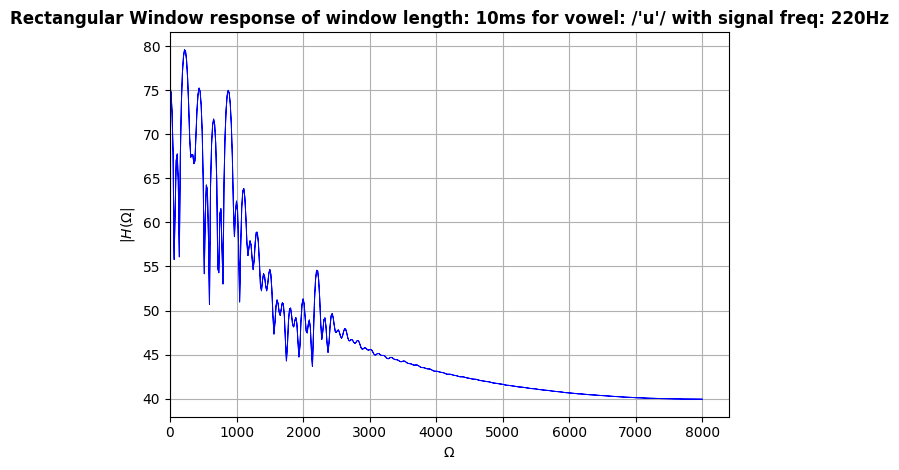
\includegraphics[scale = 0.5]{rect_10_220.png}
\caption{Rectangular Window of 10ms at Different F0}
\end{figure}
\newpage

\begin{figure}[H]
\centering
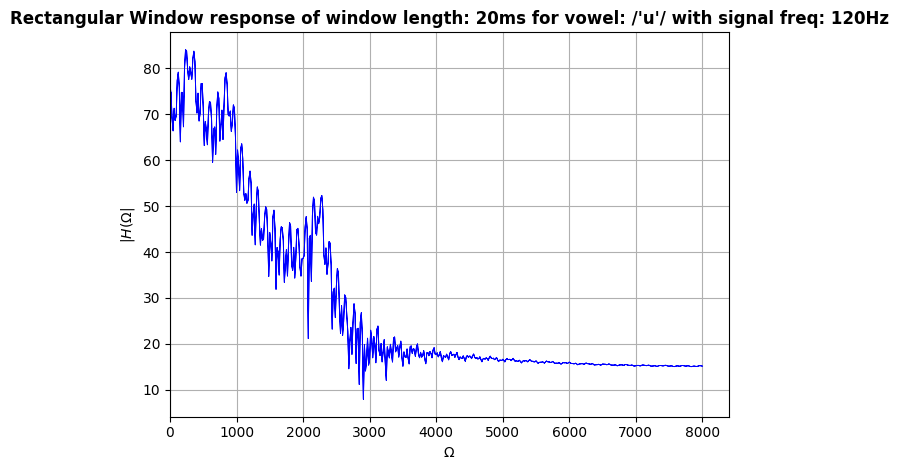
\includegraphics[scale = 0.5]{rect_20_120.png}\hfill
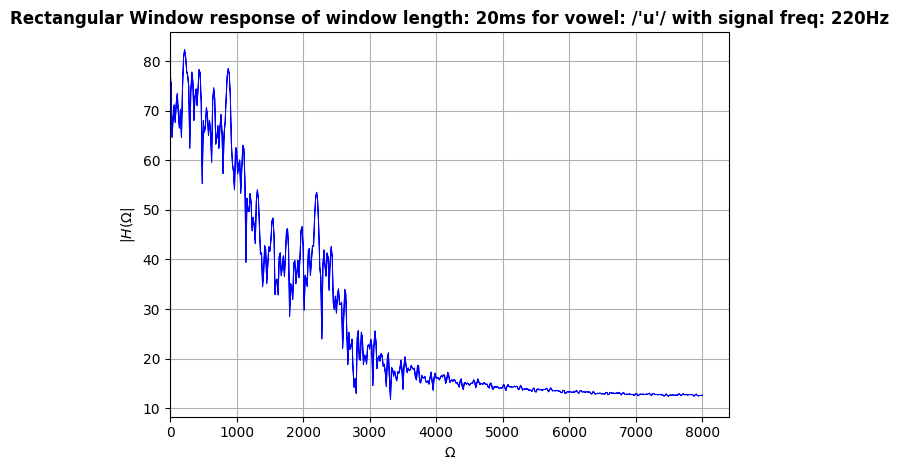
\includegraphics[scale = 0.5]{rect_20_220.png}
\caption{Rectangular Window of 20ms at Different F0}
\end{figure}

\begin{figure}[H]
\centering
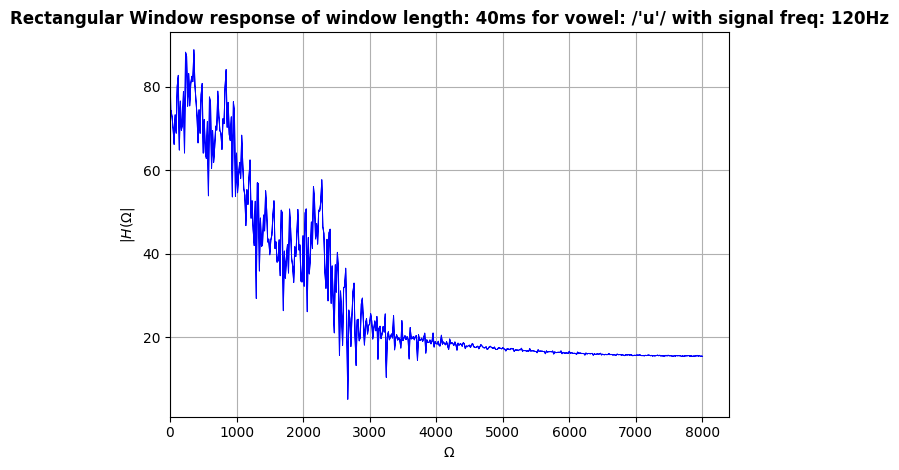
\includegraphics[scale = 0.5]{rect_40_120.png}\hfill
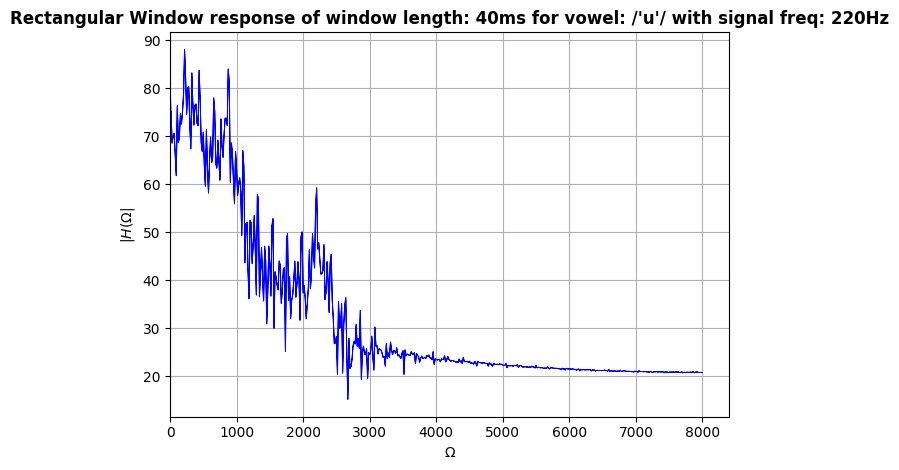
\includegraphics[scale = 0.5]{rect_40_220.png}
\caption{Rectangular Window of 40ms at Different F0}
\end{figure}
\newpage

\subsection{Results}

Firstly let's summarize the results i.e. the frequencies that we observe from the magnitude response plots of each window along with it's size in the following table. Note that all the frequencies stated below are in Hz.

\begin{center}
\captionof{table}{Comparison of Ground Truth Frequencies vs Frequencies obtained from the plots of Hamming Window for different window lengths} \label{tab:title} 
\begin{tabular}{ | c | c | c | c | c | c | c | c | c | } 
 \hline
  Ground Truth & 5ms & Difference & 10ms & Difference & 20ms & Difference & 40ms & Difference \\ 
  F0=120 & 500 & 380 & 250 & 130 & 125 & 5 & 125 & 5\\
  F1=300 & 290 & 10 & 290 & 10 & 240 & 60 & 230 & 70\\
  F2=870 & 870 & 0 & 850 & 20 & 840 & 30 & 850 & 20\\
  F3=2240 & 2230 & 10 & 2260 & 20 & 2290 & 50 & 2280 & 40\\
  \hline
  F0=220 & 500 & 380 & 250 & 30 & 250 & 30 & 250 & 30\\
  F1=300 & 300 & 0 & 230 & 70 & 230 & 70 & 220 & 80\\
  F2=870 & 870 & 0 & 880 & 10 & 880 & 10 & 880 & 10\\
  F3=2240 & 2210 & 30 & 2200 & 40 & 2190 & 50 & 2190 & 50\\
  \hline
\end{tabular}
\end{center}

\begin{center}
\captionof{table}{Comparison of Ground Truth Frequencies vs Frequencies obtained from the plots of Rectangular Window for different window lengths} \label{tab:title} 
\begin{tabular}{ | c | c | c | c | c | c | c | c | c | } 
 \hline
  Ground Truth & 5ms & Difference & 10ms & Difference & 20ms & Difference & 40ms & Difference \\ 
  F0=120 & 333 & 213 & 125 & 5 & 125 & 5 & 125 & 5\\
  F1=300 & 290 & 10 & 250 & 50 & 230 & 70 & 250 & 50\\
  F2=870 & 850 & 20 & 840 & 30 & 840 & 30 & 840 & 30 \\
  F3=2240 & 2260 & 20 & 2270 & 30 & 2270 & 30 & 2280 & 40\\
  \hline
  F0=220 & 333 & 113 & 250 & 30 & 250 & 30 & 250 & 30\\
  F1=300 & 250 & 50 & 220 & 80 & 210 & 90 & 210 & 90 \\
  F2=870 & 870 & 0 & 890 & 20 & 880 & 10 & 890 & 20\\
  F3=2240 & 2210 & 30 & 2210 & 30 & 2200 & 40 & 2190 & 50\\
  \hline
\end{tabular}
\end{center}
\newpage


\subsection{Observations}

\begin{itemize}
\item The clarity between the peak magnitudes improves if we increase the window size of either the Hamming Window or the Rectangular Window, but recognising the formant frequencies (F1, F2 and F3) becomes a little more difficult because the peaks occur very close to one another. This illustrates the switching from wide-band to narrow-band when the window size is increased.

\item As expected, the side lobes of the Hamming Window signal are quite lower than that in those where Rectangular window was applied. For a given window size, the peaks are more frequently occuring and narrowly spaced in Rectangular window setting.

\item In a given Window Function, if the fundamental frequency F0 is increased the peaks are more spaced out and the details of the waveform are more clear i.e. the peaks and in general the plot is quite smooth as compared to lower F0. 

\item The formant frequencies are simple to compute for smaller window length. The peaks accumulate to provide the precise formant frequency because of the wideband nature of the frequency response.

\item The fundamental frequency F0 is easier to calculate if we increase the window size of either the Hamming Window or the Rectangular Window. It is derived by dividing the number of high peaks occurring between 0 and 1 KHz by the frequency of 1 KHz. This can be also be seen from the results shown above that for large window length F0 is more accurate. This can also be attributed to the narrowband nature.

\item The formant frequencies are easier to calculate if we decrease the window size of either the Hamming Window or the Rectangular Window.. The peaks accumulate to provide the precise formant frequency because of the wideband nature of the frequency response. This can be also be seen from the results shown above that for shorter window length F0 is more accurate.

\item The resonating frequency of the vocal tract changes as the fundamental frequency F0 increases. The detection of the formant frequencies is also affected by this. Because for F0 = 220Hz, we can see that F2 and F3 are approximately the multiples of 220Hz, while F1 has a peak somewhere else because it is not close to a multiple of 220Hz. Similarly it can be seen for F0 = 120 Hz.

\end{itemize}



\end{document}